\documentclass[11pt, oneside]{article}

% Required packages
\usepackage[letterpaper, margin=1in, includeheadfoot]{geometry}
\usepackage{hyperref}
\usepackage{tabularx}
\usepackage{lastpage}

% Header and Footer
\usepackage{fancyhdr}
\renewcommand{\headrulewidth}{1pt}
\fancypagestyle{firstpages}{ % For first few pages
%\lhead{}\chead{\textsc{Princeton University ~~$\cdot$~~ CEE 588: Boundary Layer Meteorology ~~$\cdot$~~ J.~G.~Tylka}}\rhead{}
\lhead{\textsc{CEE 588}}\chead{\textsc{Princeton University}}\rhead{\textsc{J.~G.~Tylka}}
%\fancyhead[CO]{\textsc{CEE 588: Boundary Layer Meteorology $\cdot$ Princeton University}}
%\fancyhead[LE]{\textsc{Wind Velocity Forecasting}}
%\fancyhead[RE]{\textsc{J.~G.~Tylka}}
%\fancyhead[LO,CE,RO]{}
\lfoot{}\cfoot{\thepage}\rfoot{}
\pagenumbering{roman}
}
\fancypagestyle{pages}{ % For all other pages
\lhead{\textsc{CEE 588}}\chead{\textsc{Princeton University}}\rhead{\textsc{J.~G.~Tylka}}
\lfoot{}\cfoot{\thepage ~of \pageref{LastPage}}\rfoot{}
\pagenumbering{arabic}
}

% Additional packages
\usepackage{graphicx}
\usepackage{amssymb}
\usepackage{amsmath}
\usepackage[numbers,square,sort]{natbib}

% User-defined commands
\newcommand{\figref}[1]{Fig.~\ref{#1}}
\newcommand{\eqnref}[1]{Eq.~(\ref{#1})}
\newcommand{\eqnreftwo}[2]{Eqs.~(\ref{#1}) and (\ref{#2})}
\newcommand{\secref}[1]{Sec.~\ref{#1}}

\renewcommand{\baselinestretch}{1.5}

\begin{document}

%%%% TITLE PAGE %%%%
\begin{titlepage}
\begin{center}
~\\[1cm]
\textsc{\LARGE Princeton University}\\[1.5cm]
\textsc{\Large CEE 588: Boundary Layer Meteorology}\\[1.5cm]
\textbf{ \Large Forecasting Wind Velocity Using an Autoregressive Method}\\[1.5cm]
{\large Joseph G.~Tylka}\\
{\large \href{mailto:josephgt@princeton.edu}{josephgt@princeton.edu}}\\
\vfill
{\large Submitted: May 17\textsuperscript{th}, 2018}
\end{center}
\end{titlepage}

\pagestyle{firstpages}
%%%% ABSTRACT %%%%
\begin{abstract}
% The first sentence should be a very succinct statement of the problem; almost a rewording of the title with a few explanatory words
An autoregressive method of forecasting wind velocity is implemented and characterized.
% The second sentence should give specific motivation for the work
Autoregression is a well-established method for near-term (typically at most two days) data-driven forecasting of wind velocity, but the performance of the model depends on the timescale characteristics of the training data used to determine the coefficients of the model.
% The following 2-3 sentences should be about the adopted method and approach
Using the autocorrelation of a time-series dataset of wind velocities, relevant timescales are determined over which past wind velocities might be useful predictors of future data.
Subsequently, an autoregression model is implemented and its performance is compared, in terms of a prediction error, to the performances of two simpler predictive models: a persistence model and a random sample model.
Additionally, the performance of the autoregression model is characterized by examining the dependence of the incurred prediction errors on season and on time of day.
% The rest should be a statement of all the major findings
Results of the timescale analysis suggest that the wind system will tend to ``forget'' previous wind conditions after approximately 5.5 days.
Indeed, performance results show that, while the autoregression model performs consistently superior to the alternative models, it reaches a plateau in prediction error over approximately that timescale.
The autoregression model is also shown to yield more accurate predictions in the Summer than in the Winter, as well as during the day than at night.
\end{abstract}
\newpage
\tableofcontents
\newpage
\listoffigures

% Research questions:
% Q1: what are the relevant timescales? i.e., how far into the future must one travel to "forget" about the previous wind conditions?
% Q2: how does the autoregression method compare to persistence and random methods?
% Q3: how does the performance of the autoregression method vary with season and time-of-day?

\newpage
\pagestyle{pages}
%%%% INTRODUCTION %%%%
\section{Introduction}
% Motivation for work (from a very general perspective)
In order to facilitate the integration of wind energy into the power grid, reliable methods of forecasting wind power output are required.
% Review of previous work focusing on the remaining problems (questions or deficiencies) the present paper claims to contribute to solving
\citet{Brown1984} first proposed using autoregressive models to forecast wind power production.
However, it is unclear over what timescales an autoregression model can be expected to perform well.
Additionally, it is unclear what benefits autoregression yields over more naive approaches.
%%TODO%% flesh out literature review & motivation

% A statement of the paper's main question(s) and goal(s), followed by a succinct description of the general method and approach to be described in the paper
The primary objective of this work is to implement and characterize the performance of an autoregression model for wind velocity forecasting.
To that end, we first determine the relevant timescales over which an autoregression model can be expected to perform well by analyzing the autocorrelation of a dataset of historical wind velocities.
Subsequently, the model parameters (i.e., the autoregression coefficients) are computed using these historical wind data, and the model is evaluated using the same dataset but for a distinct (i.e., non-overlapping) time period.
This evaluation consists of randomly selecting segments of measured wind data as an input to the model, and comparing the predictions of the model to the real measurements following the input segment.
The performance of the autoregression model is compared to the performances of two simpler predictive models: a persistence model and a random sample model.
Additionally, the performance of the autoregressive model is characterized by examining the dependence of the incurred prediction errors on season and on time of day.

% A brief section by section description of the structure of the paper
The rest of this report is organized as follows.
In \secref{sec:Theory}, we review the mathematical theory used in this work.
Next, in \secref{sec:Methodology}, we describe the analyses conducted in order to determine relevant timescales and to characterize the performance of the forecasting method.
In \secref{sec:Results}, we present and discuss the results of these analyses, and finally,
in \secref{sec:Conclusions}, we summarize this work and draw conclusions from the results.

%%%% THEORY %%%%
\section{Review of Mathematical Theory}\label{sec:Theory}
In this section we first formulate the data-driven forecasting problem.
We then review four pairwise (i.e., two-point) statistics functions: the cross- and autocorrelation and cross- and autocovariance functions.
Finally, we review three forecasting methods which we will use in our analysis.

\subsection{Problem Formulation}
Consider the stream-wise and cross-stream wind velocities, $u(t)$ and $v(t)$, sampled at times $t_n$ for all integers $n$ with a sampling rate $F_s$, such that $t_n = n/F_s$.
For simplicity, we consider $t_n < 0$ to be the ``past'' and $t_n \geq 0$ to be the ``future.''
We write the wind velocity as a complex variable, $z(t) = u(t) + i v(t)$, where $i$ is the imaginary unit, and denote the sampled wind data by $u_n = u(t_n)$, $v_n = v(t_n)$, and $z_n = z(t_n)$.
The goal of data-driven wind velocity forecasting is to use past wind data, say $N_\text{in}$ previous samples, to predict $N_\text{out}$ future samples.
That is, 
\begin{equation} %%NOTE%% use "prime" notation?
\mathbf{z}_\text{out} = f(\mathbf{z}_\text{in})
\end{equation}
where $f$ is some predictive function and $\mathbf{z}_\textrm{in}$ and $\mathbf{z}_\text{out}$ are column-vectors of past and future wind data, respectively, given by
\begin{equation}
\mathbf{z}_\text{in} = 
\begin{bmatrix}
z_{-1} \\ z_{-2} \\ \vdots \\ z_{-N_\text{in}}
\end{bmatrix}
\quad\quad \text{and} \quad\quad
\mathbf{z}_\text{out} = 
\begin{bmatrix}
z_{0} \\ z_{1} \\ \vdots \\ z_{N_\text{out} - 1}
\end{bmatrix}.
\end{equation}

\subsection{Pairwise Statistics Functions}
Consider two (possibly complex-valued) sequences $X_n,Y_n$, for all integers $n \in [0,N-1]$.
Separating each sequence into two terms, the mean and the deviation from the mean, we can write
\begin{equation} %%NOTE%% revise "prime" notation
X_n = X_n' + \langle X \rangle
\quad\quad \text{and} \quad\quad
Y_n = Y_n' + \langle Y \rangle,
\end{equation}
where $\langle \cdot \rangle$ denotes taking the mean, i.e.,
\begin{equation}
\langle X \rangle = \frac{1}{N} \sum_{n = 0}^{N-1} X_n.
\end{equation}

The cross-correlation of these sequences is given by\footnote{See: \url{https://www.mathworks.com/help/signal/ref/xcorr.html}}
\begin{equation}\label{eq:xcorr}
R_{XY}(m) =
\begin{cases}
\displaystyle \sum_{n=0}^{N-m-1} X_{n+m} \overline{Y_n}, & \text{for } m \geq 0,\\[20pt]
\overline{R_{XY}}(-m), & \text{for } m < 0,
\end{cases}
\end{equation}
for all integers $m \in [-(N-1),N-1]$, where $\overline{(\cdot)}$ denotes taking the complex conjugate of the argument.
Furthermore, the autocorrelation of a single sequence, $X_n$, is given by $R_{XX}(m)$.
Note that this definition differs from that given by \citet[Sec.~8.2.1]{Stull1988}, in which the mean of the sequence is removed (cf.~\eqnref{eq:xcov} below) and a normalization factor is included.

The cross-covariance of $X_n$ and $Y_n$ is then given by\footnote{See: \url{https://www.mathworks.com/help/signal/ref/xcov.html}}
\begin{equation}\label{eq:xcov}
C_{XY}(m) = 
\begin{cases}
\displaystyle \sum_{n=0}^{N-m-1} \left( X_{n+m} - \langle X \rangle \right) \left( \overline{Y_n} - \left\langle \overline{Y} \right\rangle \right), & \text{for } m \geq 0,\\[20pt]
\overline{C_{XY}}(-m), & \text{for } m < 0,
\end{cases},
\end{equation}
which is related to the cross-correlation by $C_{XY}(m) = R_{X'Y'}(m)$, and the autocovariance of $X_n$ is given by $C_{XX}(m) = R_{X'X'}(m)$.

%%%% FORECASTING METHODS %%%%
\subsection{Forecasting Methods}\label{sec:Methods}
In this section we review three forecasting methods used in this work.
Here, we denote the measured wind velocity by $z_n$ and the predicted wind velocity by $z_n'$.

\subsubsection{Persistence}
One well-established yet inherently limited forecasting method is to use what is known as the ``persistence'' model \citep[Sec.~1.5]{Giebel2011}, wherein all future wind velocities are taken to be equal to the most recent wind velocity sample, i.e.,
\begin{equation}
z_n' = z_{-1}, \text{ for all } n \in [0, N_\text{out} - 1].
\end{equation}
Given this model's construction, we can expect (and indeed we will see in \secref{sec:Results:Comparison}) that the prediction errors incurred by this method will be small in the very near-term, but will then increase rapidly with increasing time.

\subsubsection{Random Sample}
Given a database of historical wind velocities, $\zeta_m$, for all integers $m \in [0, M-1]$, we randomly select a segment of $N_\text{out}$ consecutive samples as the predicted future samples.
That is, for some randomly selected integer $r \in [0, M - N_\text{out}]$, we take
\begin{equation}
z_n' = \zeta_{r+n}, \text{ for all } n \in [0, N_\text{out} - 1].
\end{equation}
For this method, we can expect (and again we will see in \secref{sec:Results:Comparison}) that the prediction errors will be relatively constant with time, as the randomly selected segment is likely to be largely uncorrelated with the true data.

\subsubsection{Autoregression}\label{sec:Methods:Autoregression}
An autoregression model of order $P$ uses a linear combination of the $P$ most recent time samples to predict the following one.
In general, this can be written as
\begin{equation}
z_n' = \sum_{p = 1}^P \phi_p z_{n-p},
\end{equation}
where $\phi_p$ are the autoregression coefficients for all integers $p \in [1, P]$.
In practice, this formula is applied successively to predict $z_0'$, then $z_1'$, then $z_2'$, and so forth.

Here, we compute the autoregression coefficients using a database of historical wind data $\zeta_m$ for all integers $m \in [0, M-1]$.
According to the Yule-Walker algorithm and provided that $P < M$, the autoregression coefficients are given by \citep[Sec.~3.1.1]{Chatfield2000}
\begin{equation}
\begin{bmatrix}
C_{\zeta \zeta}(1) \\
C_{\zeta \zeta}(2) \\
\vdots \\
C_{\zeta \zeta}(P)
\end{bmatrix}
=
\begin{bmatrix}
C_{\zeta \zeta}(0) & C_{\zeta \zeta}(-1) & \cdots & C_{\zeta \zeta} (-P+1) \\
C_{\zeta \zeta}(1) & C_{\zeta \zeta}(0) & \cdots & C_{\zeta \zeta} (-P+2) \\
\vdots & \vdots & \ddots & \vdots \\
C_{\zeta \zeta}(P-1) & C_{\zeta \zeta}(P-2) & \cdots & C_{\zeta \zeta}(0)
\end{bmatrix}
\cdot
\begin{bmatrix}
\phi_1 \\
\phi_2 \\
\vdots \\
\phi_P
\end{bmatrix}.
\end{equation}

Similar to the persistence model, we can expect (and again we will see in \secref{sec:Results:Comparison}) that the prediction errors incurred by this method will be small in the very near-term, but will then increase with increasing time as the wind system ``forgets'' about the previous wind conditions.

%%%% METHODOLOGY %%%%
\section{Methodology}\label{sec:Methodology}
In this work, we use a database of wind velocity measurements from the Cabauw meteorological tower,\footnote{Available for download here: \url{http://www.cesar-database.nl/Welcome.do}} which is a 213 m tall tower that has been recording, at several vertical heights, the horizontal wind speed and direction since 1986 \citep[Table I]{VanUldenWieringa1996}. %%NOTE%% what type of sensors are used?
We perform a pairwise statistical analysis of this data to determine relevant timescales, and
subsequently, we implement and characterize the three forecasting methods reviewed in \secref{sec:Methods}.

As our historical ``training'' dataset, $\zeta_m$, we use the wind velocity data measured at 200 m from January 1\textsuperscript{st}, 2001, until (and including) December 31\textsuperscript{st}, 2010.
These data are given at a sampling rate of $F_s = 6$ samples per hour.
As a pre-processing step, we first determine a nominal ``average'' direction for the wind.
To do this, we compute the wind direction $\theta_m = \arg (\zeta_m)$, where $\arg ( \cdot )$ denotes taking the argument (i.e., phase angle) of a complex number, such that $\zeta_m = |\zeta_m| e^{i \theta_m}$.
We then compute a histogram of these $\theta_m$, with a bin width of $3^\circ$, and subsequently find the peak of this histogram, which, for these data, occurs at $\hat{\theta} = -130.5^\circ$.
We then realign the training dataset and all wind data used hereafter such that
\begin{equation}
\hat{\zeta}_m = \zeta_m e^{-i\hat{\theta}}
\quad\quad \text{and} \quad\quad
\hat{z}_n = z_n e^{-i\hat{\theta}}.
\end{equation}

\subsection{Timescale Analysis}\label{sec:Methodology:Timescale}
In order to determine the timescales over which an autoregression model can be expected to perform well, we compute the autocorrelation of both $U_m$ and $V_m$, where $\zeta_m = U_m + i V_m$.
From these autocorrelation sequences, we define a timescale, $T_X$ (where $X$ can be replaced by either $U$ or $V$), given by
\begin{equation}\label{eq:Timescale}
T_X = \sum_{m = 0}^{M-1} R_{XX}(m) \Delta t,
\end{equation}
where $\Delta t = 1/F_s$.
However, in practice, we may choose to sum only over $M_\text{max}$ samples, where $M_\text{max} < M$ and is chosen based on when $R_{XX}$ reaches a sufficiently small value.
Here, we choose $M_\text{max}$ as the point at which $R_{XX}$ reaches its ``steady-state'' value, $\tilde{R}_{XX}$.

Note that since any autocorrelation sequence must decay to zero, it cannot, strictly speaking, have a non-zero ``steady-state'' value.
However, as we will see in \secref{sec:Results:Timescale}, some sequences may take a very long time to decay fully.
This might be the case, for example, when a sequence $X$ is sufficiently consistent such that its autocorrelation remains relatively constant over a wide range of $m$.
In such cases, we use a modified form of \eqnref{eq:Timescale}, such that $T_X$ is given by
\begin{equation}\label{eq:Timescale_mod}
T_X \approx \frac{1}{1 - \tilde{R}_{XX}} \sum_{m = 0}^{M_\text{max}-1} (R_{XX}(m) - \tilde{R}_{XX}) \Delta t.
\end{equation}
Note that if $\tilde{R}_{XX} = 0$, then \eqnref{eq:Timescale_mod} reduces to the unmodified \eqnref{eq:Timescale}.

\subsection{Performance Characterization}
In order to characterize the performance of the autoregression method, we first compare its performance to the performances of the other forecasting methods reviewed in \secref{sec:Methods}.
Subsequently, we investigate the dependence of the prediction errors incurred by the autoregression model on season and on time of day.

\subsubsection{Comparison of Forecasting Methods}\label{sec:Methodology:Comparison}
For each of the forecasting methods reviewed in \secref{sec:Methods}, we compute the incurred prediction errors.
To do this, we randomly select test segments of measured wind data from an ``evaluation'' dataset, for which we use the Cabauw wind data from January 1\textsuperscript{st}, 2011, until (and including) December 31\textsuperscript{st}, 2017.
Each test segment is $N_\text{in} + N_\text{out}$ samples long, where the first $N_\text{in}$ samples are given as an input to each model, and the following $N_\text{out}$ samples serve as a reference against which each model's prediction is compared.
We then compute the prediction error, $\epsilon_n = z_n - z_n'$, for all integers $n \in [0,N_\text{out}-1]$, where $z_n$ and $z_n'$ are the reference and predicted wind velocities, respectively.

We perform this calculation for $Q$ randomly selected test segments, and compute the root-mean-square (RMS) error over all test segments, given by
\begin{equation}\label{eq:RMSError}
\overline{\epsilon}_n = \sqrt{ \frac{1}{Q} \sum_{q = 1}^Q \left| \epsilon_n^{(q)} \right|^2 },
\end{equation}
where $\epsilon_n^{(q)}$ is the prediction error for the $q^\text{th}$ test segment.

\subsubsection{Seasonal and Time-of-Day Dependence}\label{sec:Methodology:SeasonalAndDiurnalDependence}
To investigate the seasonal dependence of the prediction errors, we repeat a very similar analysis to that described above in \secref{sec:Methodology:Comparison}, but restrict the randomly selected test segments to be from a given season.
In particular, we ensure that the entire test segment is contained within the same season.
Similarly, to investigate the dependence on the time of day, we restrict the randomly selected test segments such that the reference wind velocity segments are no longer than 12 hours and are either daytime (starting at 8AM) or nighttime (starting at 8PM) segments.

%%%% RESULTS %%%%
\section{Results and Discussion}\label{sec:Results}
In this section we present and discuss the results of the analyses described above.

\subsection{Timescale Analysis}\label{sec:Results:Timescale}
In \figref{fig:Autocorrelations}, we plot the autocorrelation sequences $R_{UU}(m)$ and $R_{VV}(m)$, which have been normalized such that $R_{UU}(0) = R_{VV}(0) = 1$.
From this plot, we see that $R_{UU}$ reaches its ``steady-state'' value of approximately $\tilde{R}_{UU} = 0.1$ after approximately 70 days.
In contrast, the steady-state value of $R_{VV}$ is essentially $\tilde{R}_{VV} = 0$ and is reached after approximately 15 days.
Choosing $M_\text{max}$ as the first (i.e., smallest positive) value of $m$ at which $R_{XX}(m) < \tilde{R}_{XX}$, we compute, using \eqnref{eq:Timescale_mod}, the timescales $T_U$ and $T_V$.
For each curve in \figref{fig:Autocorrelations}, the area between $\tilde{R}_{XX}$ and $R_{XX}(m)$ is shaded for $m < M_\text{max}$, corresponding to the value of the summation in \eqnref{eq:Timescale_mod}.

\begin{figure}[htb]
\centering
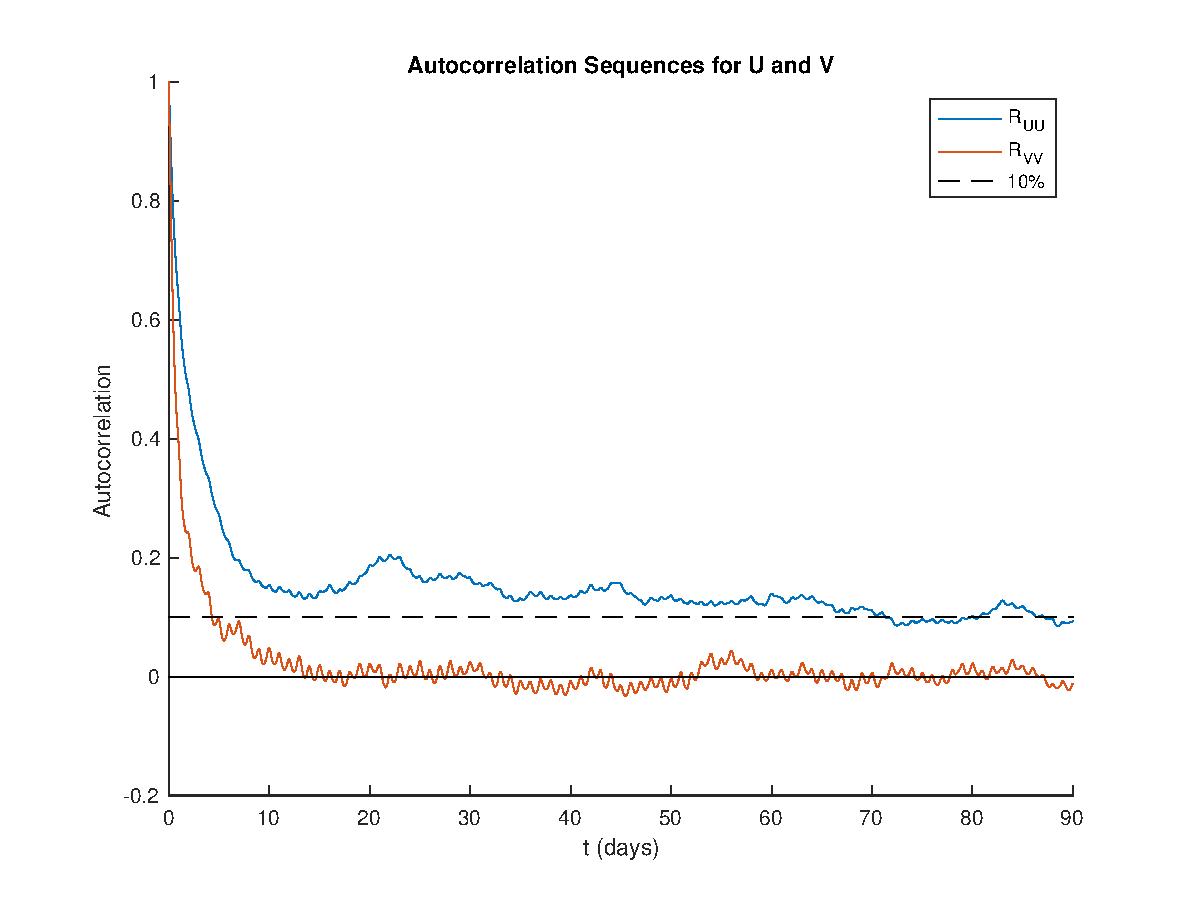
\includegraphics[width=0.7\columnwidth]{figures/AutocorrelationSequences_90days}
\caption{Normalized autocorrelation sequences $R_{UU}$ (blue curve) and $R_{VV}$ (red).
The filled regions correspond to the summations computed using \eqnref{eq:Timescale_mod} to find the timescales $T_U$ and $T_V$.}
\label{fig:Autocorrelations}
\end{figure}

We find the timescales computed with \eqnref{eq:Timescale_mod} to be $T_U \approx 5.44$ days and $T_V \approx 1.71$ days.
These values suggest that the stream-wise winds tend to remain correlated for $\sim 5.5$ days, while the cross-stream winds remain correlated for only $\sim 2$ days.
Consequently, we can expect the errors incurred by the autoregression and persistence models to attain relatively constant values after $\sim 5.5$ days. %%NOTE%% does this agree with knowledge?

\subsection{Performance Characterization}
Here, we construct an autoregression model, as described in \secref{sec:Methods:Autoregression}, with an order $P$ corresponding to 2 days, i.e., $P = 2 \times 24 F_s$, where $F_s$ is given in samples per hour.
In each analysis below, we have computed, using \eqnref{eq:RMSError}, the RMS error averaged over $Q = 100$ test segments.

\subsubsection{Comparison of Forecasting Methods}\label{sec:Results:Comparison}
The RMS prediction errors incurred by each forecasting method are plotted in \figref{fig:ComparisonRMS}.
Here, we take $N_\text{in}$ and $N_\text{out}$ to correspond to 2 and 30 days, respectively.
From this plot, we see that the autoregression method performs consistently superior to both the persistence and random sample methods.

\begin{figure}[htb]
\centering
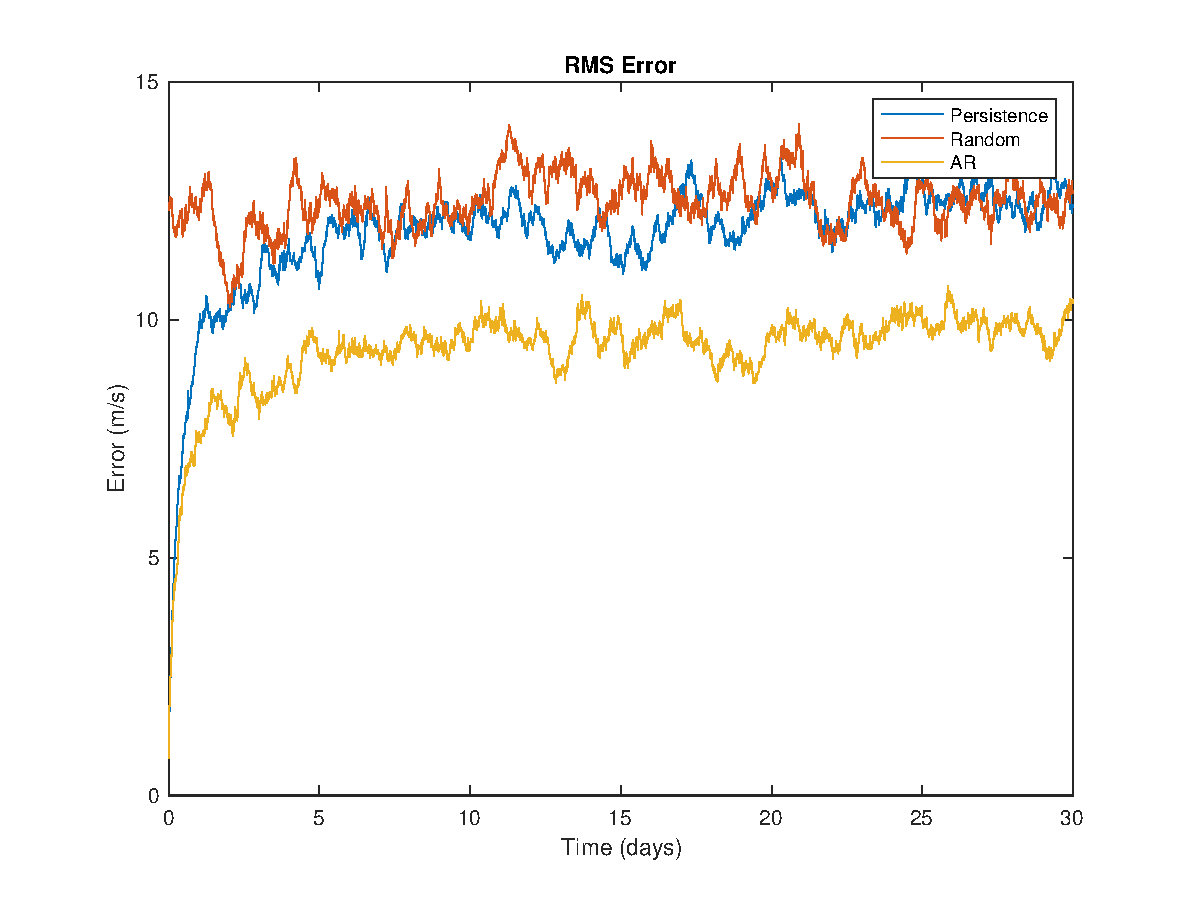
\includegraphics[width=0.7\columnwidth]{figures/ComparisonRMSPredictionError}
\caption{Comparison of RMS prediction errors incurred by the persistence (blue curve), random sample (red), and autoregression (green) models.
The horizontal dashed red line indicates the average (mean) value of the RMS error for the random sample model (equal to approximately 12.5 m/s).
The vertical dashed lines indicate 2 and 5.5 days.}
\label{fig:ComparisonRMS}
\end{figure}

As expected, we see that the RMS errors incurred by the random sample model are approximately constant with $n$.
For the persistence model, however, we see that the RMS errors are small at small $t_n$, but ultimately reach similar values to those incurred by the random sample model.
We interpret this behavior as corresponding to the system ``forgetting'' about the previous wind conditions, and, in particular, we see that this happens when $t_n \approx T_U \sim 5.5$ days.

Similarly, we see that the autoregression model reaches a similar plateau in RMS error beyond $T_U$.
However, these errors are still smaller than those of the persistence and random sample models.
This suggests that, even though the system has ``forgotten'' about the previous wind conditions, the autoregression model is still able to achieve predictions that are \textit{slightly} more accurate than the totally independent predictions produced by the alternative methods.
Although not shown here, it can be verified that these plateaus remain constant even when forecasting up to 365 days into the future. %%NOTE%% show this?

\subsubsection{Seasonal and Time-of-Day Dependence}
The RMS prediction errors incurred in each season by the autoregression model are plotted in \figref{fig:SeasonalRMS}.
From this plot, we see that the errors are smallest in the Summer and largest in the Winter.
This suggests that wind conditions in Spring and Summer tend to be ``more predictable'' than those in Fall or Winter. %%TODO%% talk more about this?

\begin{figure}[htb]
\centering
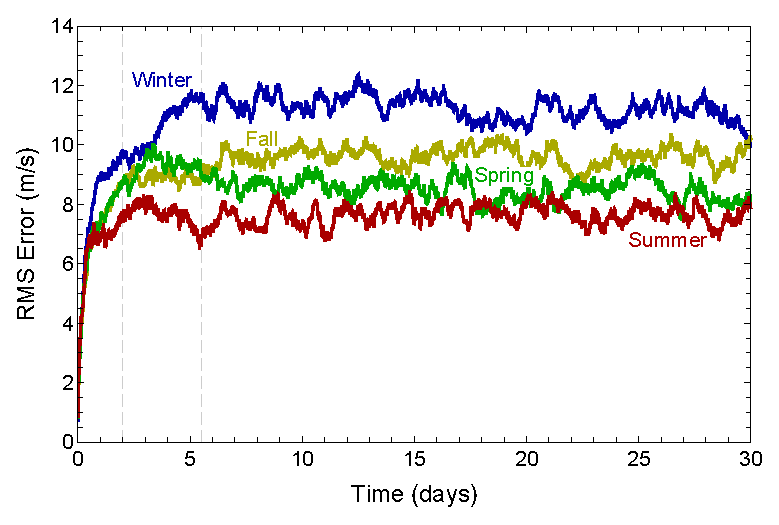
\includegraphics[width=0.7\columnwidth]{figures/SeasonalRMSPredictionError}
\caption{Seasonal dependence of RMS prediction errors incurred by the autoregression method.
The vertical dashed lines indicate 2 and 5.5 days.}
\label{fig:SeasonalRMS}
\end{figure}

The RMS prediction errors incurred under daytime and nighttime conditions by the autoregression model are plotted in \figref{fig:DiurnalRMS}.
From this plot, we see that the prediction errors incurred during the day are consistently smaller than those incurred at night.
This is somewhat surprising, as we might expect nighttime conditions to be ``more predictable'' due to the stability of the atmospheric boundary layer \citep[Fig.~1.7]{Stull1988}.
However, these results suggest that the autoregression method is better able to predict daytime wind conditions given data from the previous night, than it is to predict nighttime wind conditions given data from the previous day.
Consequently, we infer that nighttime wind conditions are more useful predictors of the following day's winds than the opposite. %%TODO%% revise language here - slight improvement

\begin{figure}[htb]
\centering
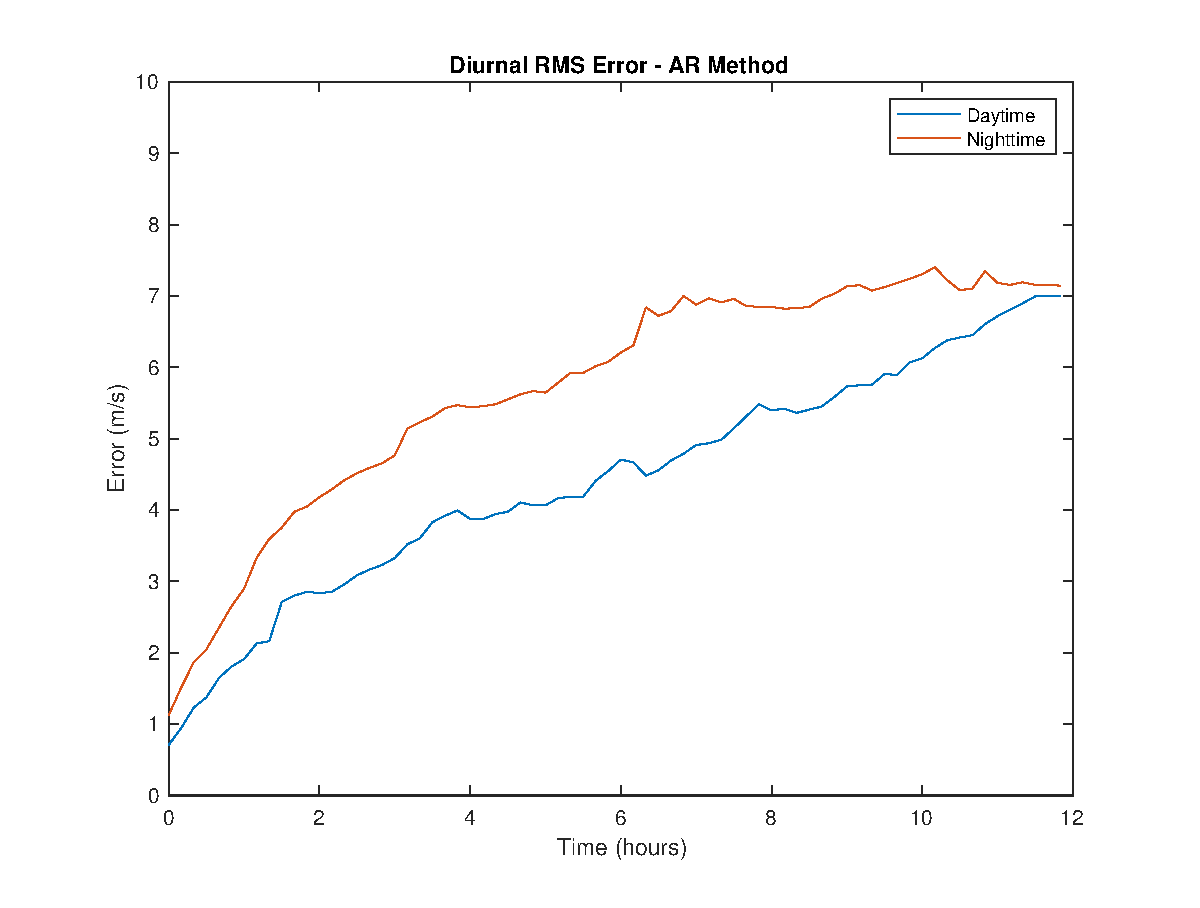
\includegraphics[width=0.7\columnwidth]{figures/DiurnalRMSPredictionError}
\caption{Time-of-day dependence of RMS prediction errors incurred by the autoregression method.
For daytime predictions (red curve), $t = 0$ corresponds to 8AM, while for nighttime predictions (blue), $t = 0$ corresponds to 8PM.}
\label{fig:DiurnalRMS}
\end{figure}

%%%% CONCLUSIONS %%%%
\section{Summary and Conclusions}\label{sec:Conclusions}
In this work we implemented and characterized the performance of an autoregression model for wind velocity forecasting.
We first determined the relevant timescales over which an autoregression model can be expected to perform well by analyzing the autocorrelation of a dataset of historical wind data.
Subsequently, we compared, in terms of an average prediction error, the performance of the autoregression model to the performances of two simpler predictive models: a persistence model and a random sample.
Additionally, we examined the dependence of the incurred prediction errors on season and on time of day.

Results of the timescale analysis suggest that the wind system will tend to ``forget'' previous wind conditions after approximately 5.5 days (see \secref{sec:Results:Timescale}).
Indeed, results show that, while the autoregression model performs consistently superior to the simpler alternative models, it reaches a plateau in prediction error over approximately that timescale (see \figref{fig:ComparisonRMS}).
The autoregression model was also found to yield more accurate predictions in the Summer than in the Winter (see \figref{fig:SeasonalRMS}), which suggests that wind conditions in the Summer may be more consistent and ``predictable'' as a result.
Daytime predictions of wind velocity were also found to be more accurate than nighttime predictions (see \figref{fig:DiurnalRMS}), which suggests that nighttime wind conditions are more useful predictors of the following day's winds than the opposite.

\subsection{Future Work}
Future investigations should include an implementation of more specific or localized autoregression models.
For example, different autoregression coefficients might be computed for each season or for each time of day.
Additionally, the performance of the autoregression model should be compared to numerical weather prediction models, such the Weather Research and Forecasting model,\footnote{Available for download here: \url{https://www.mmm.ucar.edu/weather-research-and-forecasting-model}} which have been shown to perform better than persistence beyond about 6 hours \citep{Giebel2011,LandbergWatson1994}.

\addcontentsline{toc}{section}{References}
\bibliographystyle{unsrtnat}
\bibliography{refs}

\end{document}